%!TEX root = ../../main.tex
\chapter{序論}
\label{chap:intro}

\section{本研究の背景}
音楽知識や音楽経験に乏しい人が音楽によるインタラクションを試みる際,調性感を損なわない音を発して参加することは非常に困難である.
実際に音楽未経験者が自由にかつ能動的に音楽インタラクションに参加する場合として,
地域社会振興のために開催される音楽イベント,アーティストのコンサート,などが考えられる.
従来,音楽経験の乏しい人がそのようなパフォーマンスに参加する手段は手拍子や掛け声,リズムに合わせて体を動かす程度のことに限られている,
波多野\cite{hatano2007}は旋律歌唱能力の発達過程や旋律聴取の認知的処理における3つの処理側面として,図\ref{img:hatano}に示すように,(1)リズム(rhythm),(2)旋律線(pitch contour),(3)調性(tonality)があるとしている.
(2)の旋律線とは音高の上がり下がりの運動パターンのことであり,初心者でもリズムやおおまかになら音が上がったか下がったかは比較的理解しやすい.(3)の調性とは文献\cite{ongakunotomo1979}によれば,広義には「支配的な中心音を有する音楽系」を指し,狭義には「長短調いずれかの主和音をもつ和声的な音楽系」を指す.調性は中心音,長調/短調,音階,和音などから説明され,音楽初心者が音楽について学ぼうとする場合,調性を理解することは最も大きな障害のひとつである.
よって調性は音楽未経験者が音楽活動を行おうとする際,苦手意識を持たれる原因となる.
この調性に関する知識の無さが引き起こす問題点を解決することで,誰でもより充実した音楽活動をすることが容易になると考えた.

\begin{figure}[t]
	\begin{center}
		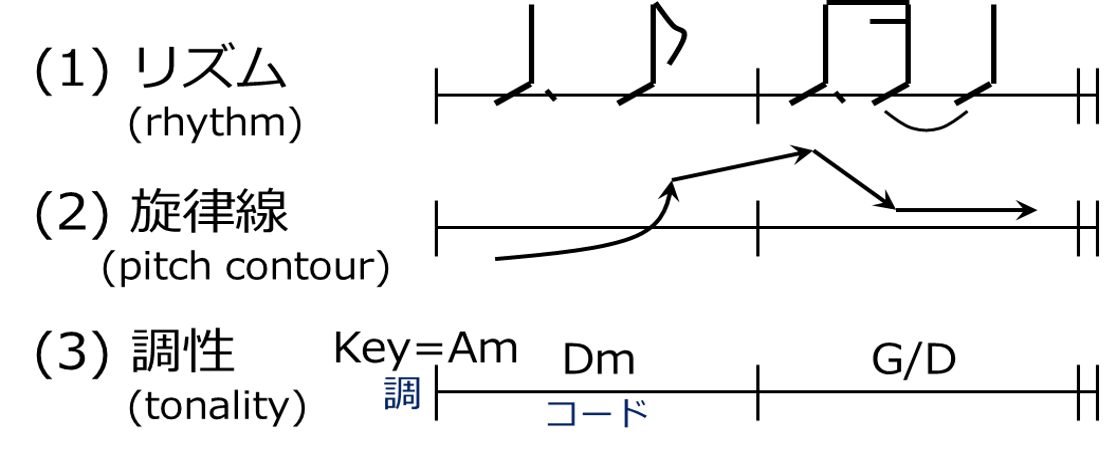
\includegraphics[width=0.9\linewidth]{assets/img/hatano.png}
		 \caption{旋律歌唱や旋律聴取の認知的処理における3つの処理側面}
		\label{img:hatano}
	\end{center}
\end{figure}
\section{本研究の目的}
本研究の目的は,ユーザーが直感的に操作できるように比較的知識を必要としないリズムと旋律線を身体動作で入力すれば,システムの音高補正により背景で流れている楽曲との調性の制約(以下,調性制約)に従って背景楽曲と協和を満たす演奏音を出力することで,音楽知識がなくても合奏ができる演奏インタフェースの実現である. 菅\cite{suga2008}は旋律線の手なぞりなどの身体動作が音楽理解を促進する方法として有効であるとしている.そのため旋律線の入力手段として身体動作を用いることは適切である.
本研究完成時には調性感を共有した演奏参加が可能になると期待される.コンサート会場で演奏される実楽曲の調や旋法と同期させた使い方を考えると,ステージ上のアーティストと聴衆のインタラクションのあり方を変える可能性があり,さらに,学校・保育施設での情操教育や福祉施設でのリハビリテーションにも活用できる可能性があり,幼児,児童,高齢者などのQOL向上に繋がると期待される.
また,旋律線とリズムを身体動作で入力することにより,ユーザーは演奏のための楽器を持ち運ぶ必要がなくなるため,演奏場所への移動距離や,スペースの制約に縛られることがない.
その操作性と音高の決定手法においていくつかの問題点ある.本研究ではそれらの問題を
(1)直感的な身体動作による旋律線やタイミング,音の種類などの入力手法.(2)演奏音の発音可能な音高範囲の指定.(3)調性制約の生成.の3つの課題として設定した.
\subsection{システム構成}
本システムのシステム構成を図\ref{img:sys_const}に示す.
まず,ユーザーはモーションセンサーの前でリズムと旋律線を身体動作で入力する.本研究ではモーションセンサーはIntel RealSense 3D Camera\footnote{http://www.intel.co.jp/content/www/jp/ja/architecture-and-technology/realsense-overview.html} (以下,RealSense)を使用した,RealSenseは手指の情報とジェスチャーを検出し,認識結果を本研究で実装する合奏支援システムに渡す.システム内部ではジェスチャーによるイベント切り替えや,手の座標とあらかじめ用意しておいた調性制約から背景楽曲と不協和音にならない演奏音を出力する.
\begin{figure}[t]
	\begin{center}
		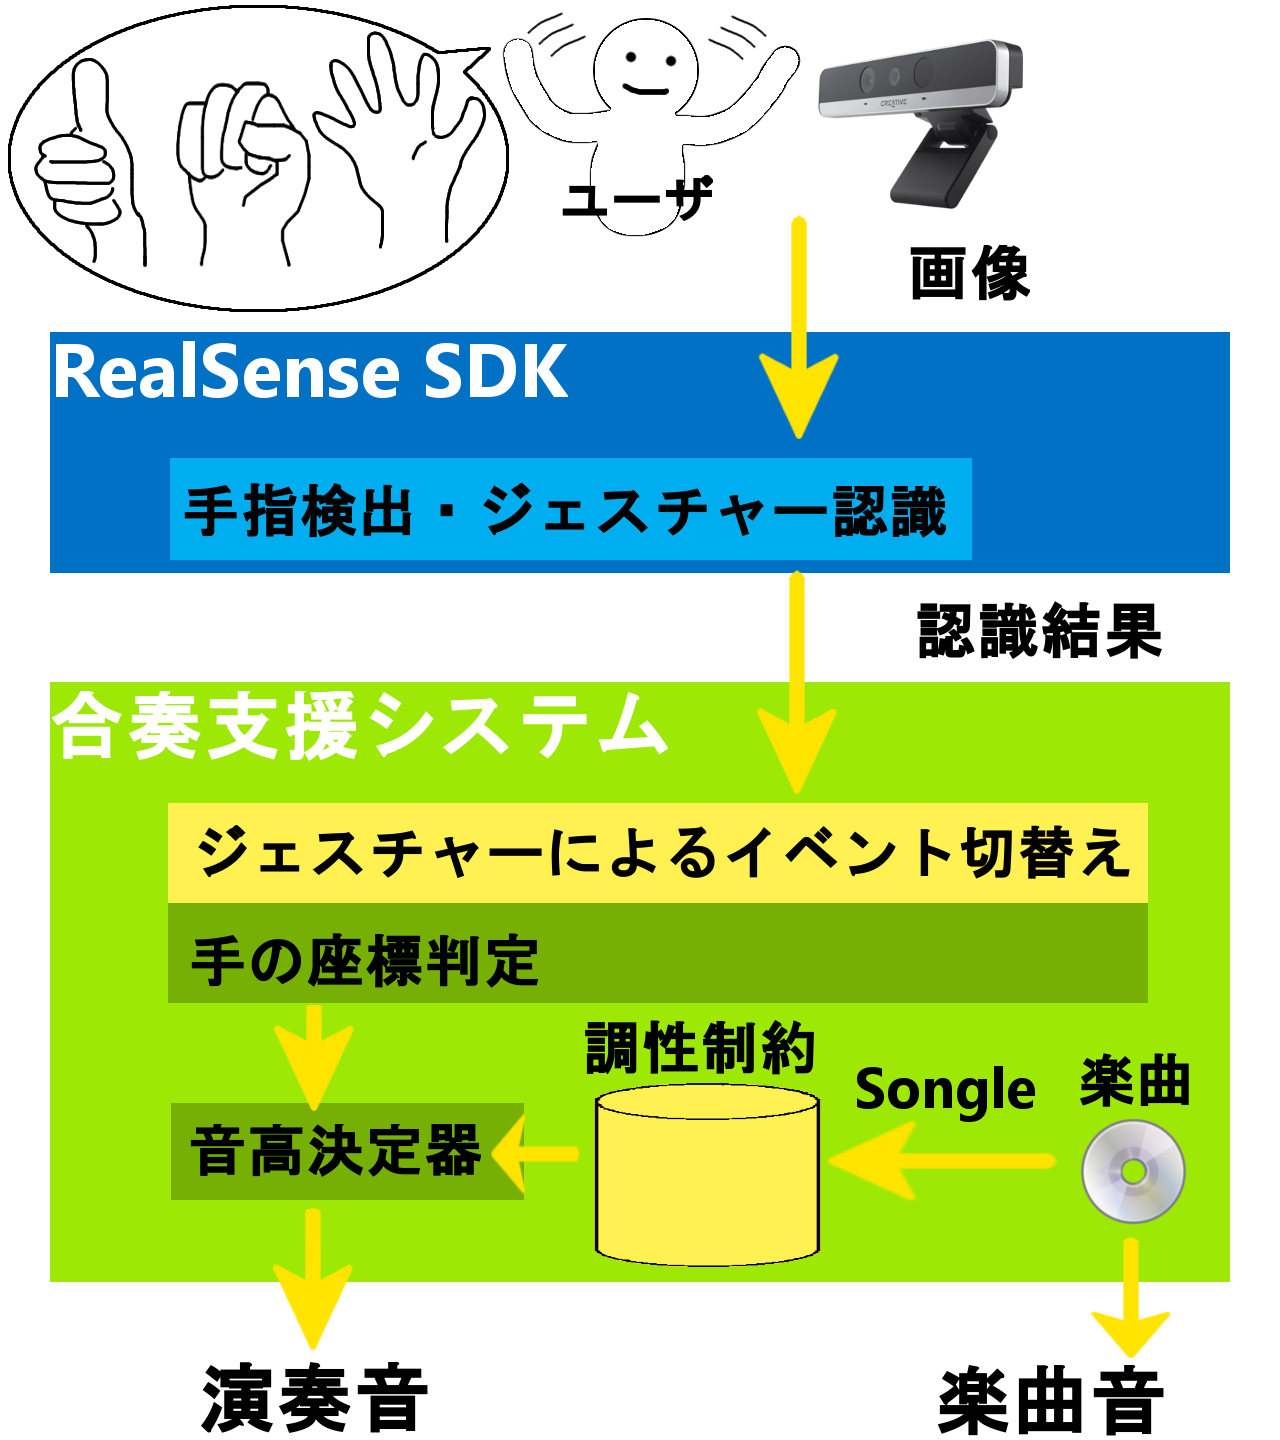
\includegraphics[width=0.9\linewidth]{assets/img/system_configuration_diagram.png}
		\caption{システム構成図}
		\label{img:sys_const}
	\end{center}
\end{figure}
\section{本論文の構成}
本論文の構成を以下に示す.第2章では関連研究や関連システムと本研究の動作・開発環境について述べる.第3章では直感的な身体動作とリズムの入力手法について述べる.第4章では演奏音の発音可能な音高範囲の指定について述べる.第5章では調性制約の生成について述べる,第6章では前章までで述べたシステムの評価実験の結果をまとめ,第7章で本研究をまとめる.
